
\subsection*{1.}

L'arbre pondéré ci-dessous représente une situation où \(A\), \(B\), \(C\) et \(D\) sont des événements d'une expérience aléatoire :

\begin{center}
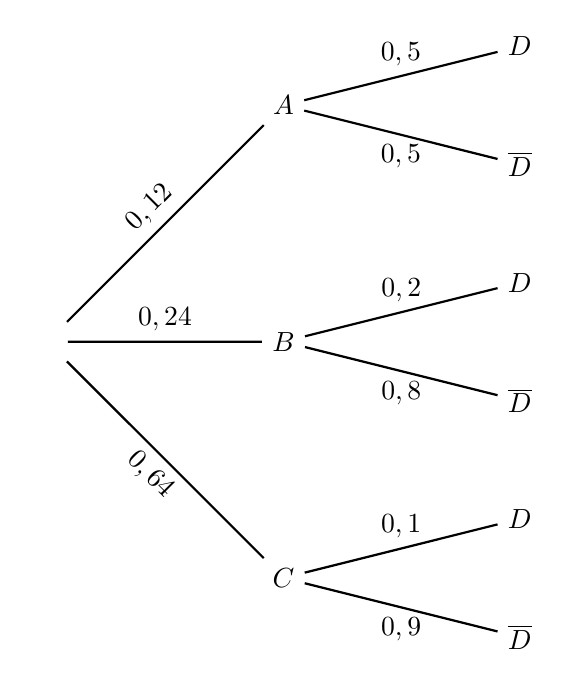
\begin{tikzpicture}[thick, scale=1.5]
\node (P_-1_0) at (-2,-2.5) {$\phantom{A}$};
\node (P_0_0) at (0,-0.5) {$A$};
\draw (P_-1_0) -- (P_0_0) node[midway, above,sloped] {$0,12$};
\node (P_1_0) at (2,-0) {$D$};
\draw (P_0_0) -- (P_1_0) node[midway, above] {$0,5$};
\node (P_1_1) at (2,-1) {$\overline{D}$};
\draw (P_0_0) -- (P_1_1) node[midway, below] {$0,5$};
\node (P_0_2) at (0,-2.5) {$B$};
\draw (P_-1_0) -- (P_0_2) node[midway, above] {$0,24$};
\node (P_1_2) at (2,-2) {$D$};
\draw (P_0_2) -- (P_1_2) node[midway, above] {$0,2$};
\node (P_1_3) at (2,-3) {$\overline{D}$};
\draw (P_0_2) -- (P_1_3) node[midway, below] {$0,8$};
\node (P_0_4) at (0,-4.5) {$C$};
\draw (P_-1_0) -- (P_0_4) node[midway, below,sloped] {$0,64$};
\node (P_1_4) at (2,-4) {$D$};
\draw (P_0_4) -- (P_1_4) node[midway, above] {$0,1$};
\node (P_1_5) at (2,-5) {$\overline{D}$};
\draw (P_0_4) -- (P_1_5) node[midway, below] {$0,9$};
\end{tikzpicture}
\end{center}

D'après la loi des probabilités totales :

\(
p(D) = p(A \cap D) + p(B \cap D) + p(C \cap D),
\)

\(
p(D) = p(A) \times p_A(D) + p(B) \times p_B(D) + p(C) \times p_C(D),
\)

\(
p(D) = 0,12 \times 0,5 + 0,24 \times 0,2 + 0,64 \times 0,1 = 0,06 + 0,048 + 0,064 = 0,172.
\)

\subsection*{2.}

Pour le trinôme \(-2x^2 - 5x + 3\), on a :
\(
\Delta = 25 + 4 \times 2 \times 3 = 25 + 24 = 49 = 7^2 > 0.
\)

Ce trinôme a deux racines :
\(
x_1 = \dfrac{5 + 7}{-4} = -3 \quad \text{et} \quad x_2 = \dfrac{5 - 7}{-4} = \dfrac{1}{2}.
\)

On sait que ce trinôme est négatif sauf sur l'intervalle \(\left] -3 \,;\, \dfrac{1}{2} \right[\).

Donc :
\(
S = \left] -\infty \,;\, -3 \right[ \cup \left] \dfrac{1}{2} \,;\, +\infty \right[.
\)

\subsection*{3.}

Un vecteur directeur de la droite a pour coordonnées \(\begin{pmatrix} 8 \\ 2 \end{pmatrix}\),
donc un vecteur normal a pour coordonnées \(\begin{pmatrix} -2 \\ 8 \end{pmatrix}\) ou \(\begin{pmatrix} 1 \\ -4 \end{pmatrix}\).

\subsection*{4.}

\begin{align*}
&M(x\,;\,y) \in \mathcal{C}(A\,;\,R = 2)\\
\iff& (AM^2 = 2^2\\
\iff &(x - (-2))^2 + (y - (-4))^2 = 4\\
\iff &(x + 2)^2 + (y + 4)^2 = 4\\
\iff &x^2 + 4 + 4x + y^2 + 16 + 8y = 4\\
\iff &x^2 + y^2 + 4x + 8y + 16 = 0
\end{align*}

\subsection*{5.}

On a effectivement :
\[
u_1 = u_0 + 2 \times 0 - 3 = 1 + 0 - 3 = -2,
\]
\[
u_2 = u_1 + 2 \times 1 - 3 = -2 + 2 - 3 = -3.
\]

